\documentclass[12pt,letterpaper]{article}
\usepackage[utf8]{inputenc}
\usepackage{makeidx}
\usepackage{graphicx}
\usepackage{lmodern}
\usepackage[left=1in,right=1in,top=1in,bottom=1in]{geometry}
\author{Sean Gallagher, Hossein Hemati, Wlodek Zadrozny}
\title{Progress on Extraction of Medical Guidelines}
\begin{document}
\maketitle
\begin{abstract}
Our objective in the project has thus far been to show that we can extract medical information from text, particularly medical guidelines from text. In doing this, we have taken three approaches, building links from analysis of constituent trees, building links from regular expression matches on plain text, and via answer type detection in an existing question answering system.
\end{abstract}
\section{Constituent Trees}
Our first attempt at extracting medical conditions and symptoms from unstructured text is by using heirarchical analysis of a constituent parse tree of the text. The system is relatively simple, following a general pattern:

\begin{enumerate}
\item Decend to the leaves of the tree, the original words.
\item Match classes of words for operators and numeric values.
\item Match the remaining words against known tests and diseases.
\item Ascend the tree, combining analyses as follows:
\begin{itemize}
	\item A decimal value, an operator, and a test constitute a condition.
	\item A condition and an ailment constitute a link, which is the program output.
\end{itemize}
\end{enumerate}

There are several concerns about this approach, not the least of which are the limited scope of the links it can extract. It expects guidelines of the form
"Values of $A1C \geq 6.5$ may indicate diabetes," but this causes serious brittleness. Consider the generally equivalent statement: "A1C values predict diabetes when greater than approximately 6.5."

There are also weaknesses with tables, which are relatively common in medical literature, and any document of such links. Take for example the Wikipedia article on Diabetes. The condition information is stored in a structured way, as a table. The trouble is that it is not clear how to interpret the contents. "$\geq 6.5$" can be interpreted as a operator and value. But the rest of the content needs more context, and this is what we are aiming to solve in section three.
\begin{figure}
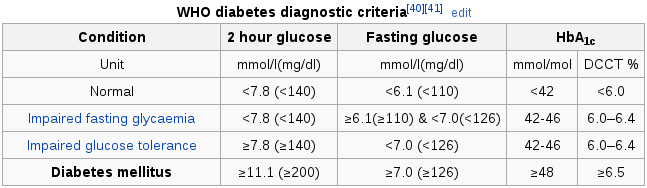
\includegraphics[width=\textwidth]{WikipediaA1CTable}
\caption{Excerpt of the Wikipedia article on Diabetes}
\end{figure}
\section{Regular Expressions}
\section{Dependency Graphs}
% Integrated into Watsonsim
We aim to improve our recognition of diagnostic criteria using other knowledge also available on Wikipedia. We can do that with many of the tools we have already been developing for question answering with Watsonsim.

Firstly, rather than hard-coding the names of many diseases we want to detect, we can recognize the types of the words we encounter using answer type detection. This way our approach will generalize better for new diseases.
Secondly, we can use many Wikipedia sources to determine semantic relations between phrases. For example, we have determined that $HbA_{1c}$, as seen in the excerpt given above, is a synonym for the main article "Glycated hemoglobin." We do this by keeping a table of the redirects between Wikipedia articles. We also assume that phrases which label a link to an article are synonymous with the title of the target article, and we use this to measure synonymy.

\subsection{Lexical Answer Types}
% Tried conceptnet
% Investigating NELL
On the outset we intended to use DBPedia to detect answer types, but these are not usually specific enough to be greatly helpful, and are synonymous with the target type only on very rare occasions. We attempted to supplement this using ConceptNet, but our initial tests, before parsing the entire knowledge base, still do not indicate very high recall rates. Instead, we have developed a simple rule-based method of extracting lexical answer types from supporting passages. This covers many cases and are reasonably specific but in several instances they make unnecessary distinctions. (Sign and symptom may often be used interchangably, even though Wikipedia makes a distinction; we have noted similar situations with writer and author.) At any rate, we are examining whether to include the NELL ontology, which does at least contain many of the phrases we are targeting.

Nonetheless, there are situations where knowing the exact type of a referent is not immediately helpful. Going back to the previous example, there is no direct statement that glycated hemoglobin is a medical test in the following passage, because it is actually the subject of an implied test of its quantity:
\begin{quote}
Glycated hemoglobin (hemoglobin A1c, HbA1c, A1C, or Hb1c; sometimes also HbA1c or HGBA1C) is a form of hemoglobin that is measured primarily to identify the average plasma glucose concentration over prolonged periods of time.
\end{quote}
This is not immediately helpful because it is not yet clear that glycated hemoglobin is the subject of any test. Unless NELL or a similar ontology has this information, some other general solution for reading such tables will need to be found, or else they may need to be handled more manually.

% Could also build an ontology from reading
\subsection{Link Expansion}
When evaluating supporting passages to discover answer types, we have found it useful to annotate more than just the answer the passage supports. Finding a new object with the correct LAT but in a supporting passage for another candidate answer now triggers the generation of new candidate answers.

The intuition for such an inclusion is clear. The symptom of pain is relevant enough to diabetes for authors to choose to include it, but diabetes is not relevant enough to pain for the inverse to occur. As a result, any list of symptoms or conditions relating to diabetes will be incomplete unless the evidence for an answer comes in large part from outside of its article.

The new implications of the LAT search has the curious effect that the text analysis pipeline operates as a tree when a detected LAT suggests a new candidate. We believe we can further stimulate this effect by then running LAT detection on the newly generated candidate answers, making a pipeline a graph, but the appropriate termination conditions are as yet unclear.
% Pull pipeline
% Mention redirects
% Say, using real links rather than redirects
\end{document}